\documentclass[a4paper,UTF8]{ctexart}

\usepackage{amsmath, amsthm, amssymb, amsfonts, hyperref, mathrsfs}%美国数学学会的包+?
\usepackage{geometry} %控制界面
\usepackage{bookmark}
\usepackage{fancyhdr} % header & footer
\usepackage{appendix} % 附录
\usepackage{tikz} %作图
\usepackage{graphicx} %插入图片的宏包
\usepackage{float} %设置图片浮动位置的宏包
%\usepackage{subfigure} %插入多图时用子图显示的宏包
\usepackage{listings} %引用代码
\usepackage{physics,mathtools} %物理数学工具
\usepackage{comment}
\usepackage{framed}
\usepackage{caption}
\usepackage{subcaption}
\geometry{top=2.5cm,bottom=2.5cm,left=2.5cm,right=2.5cm} % 布局要求
\pagestyle{fancy} % fancy分格
\fancyhf{} % 清除所有页眉页脚
\renewcommand\headrulewidth{0.6pt}
\renewcommand\footrulewidth{0.6pt}
% font
\setCJKmainfont{Noto Serif CJK SC}[BoldFont={Noto Serif CJK SC Bold}, ItalicFont=]
\lhead{何金铭 PB21020660$\mid$座位号:1}
\cfoot{高阶涡旋光束的产生与检测实验报告附录}
\rhead{\thepage}
\lfoot{2024.4.17}
\rfoot{USTC}
%\bibliographystyle{plain} % 引用样式
\everymath{\displaystyle} % display
%============================================================

\begin{document}

\begin{center}
    \textbf{\Large 高阶涡旋光束的产生与检测实验报告附录}
    \par \text{\large 何金铭 PB21020660}
\end{center}

\section{柱矢量光束光强分布}

\begin{figure}[H]
    \centering
    \begin{minipage}[b]{0.9\textwidth}
        \centering
        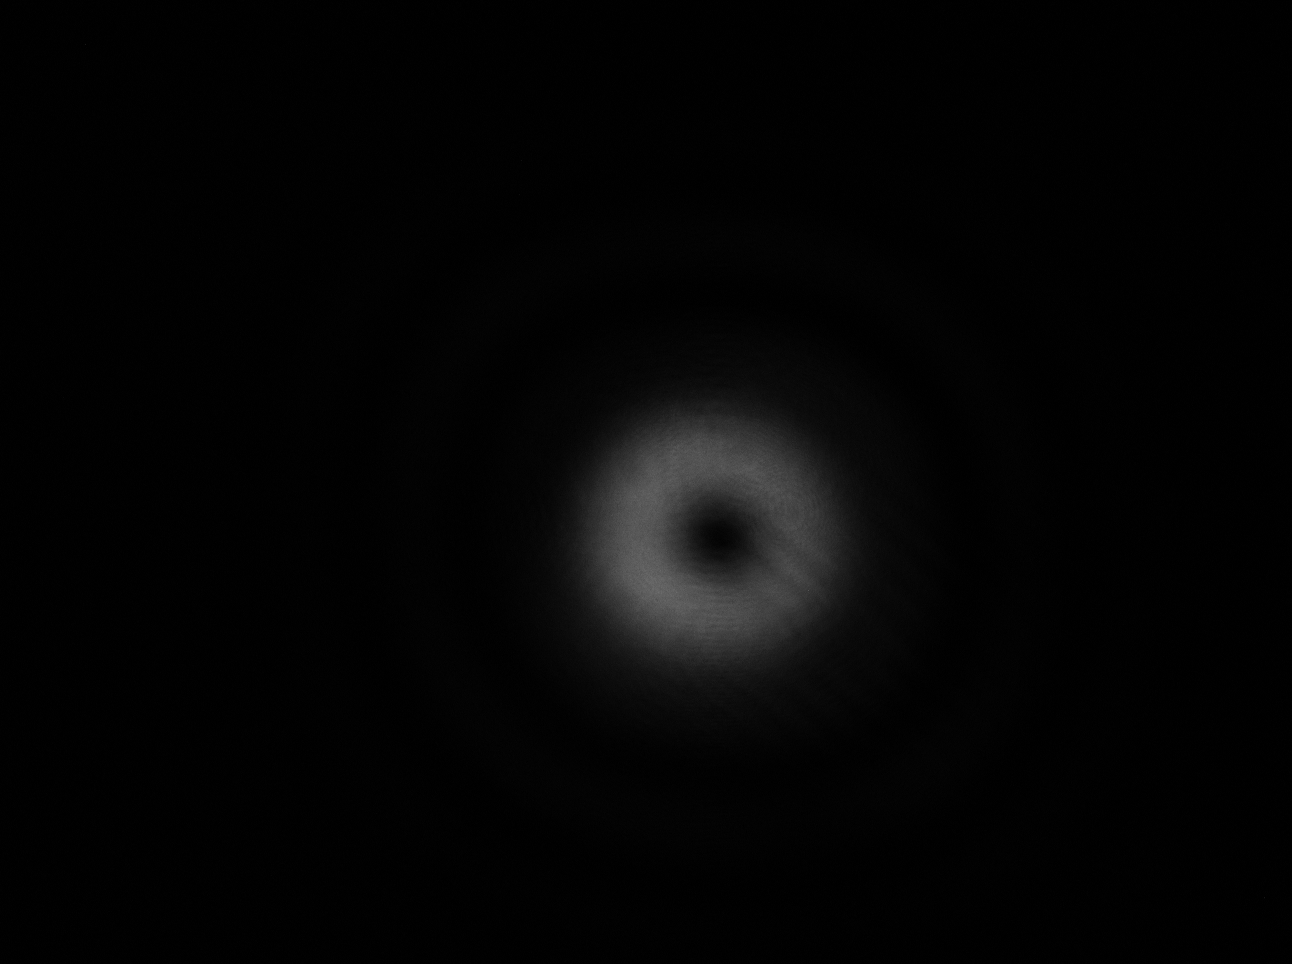
\includegraphics[width=0.7\textwidth]{./fig/1.png}
        \caption{柱矢量光束光强分布}
    \end{minipage}
\end{figure}

\subsection{径向偏振光检偏}

\begin{figure}[H]
    \centering
    \begin{minipage}[b]{0.45\textwidth}
        \centering
        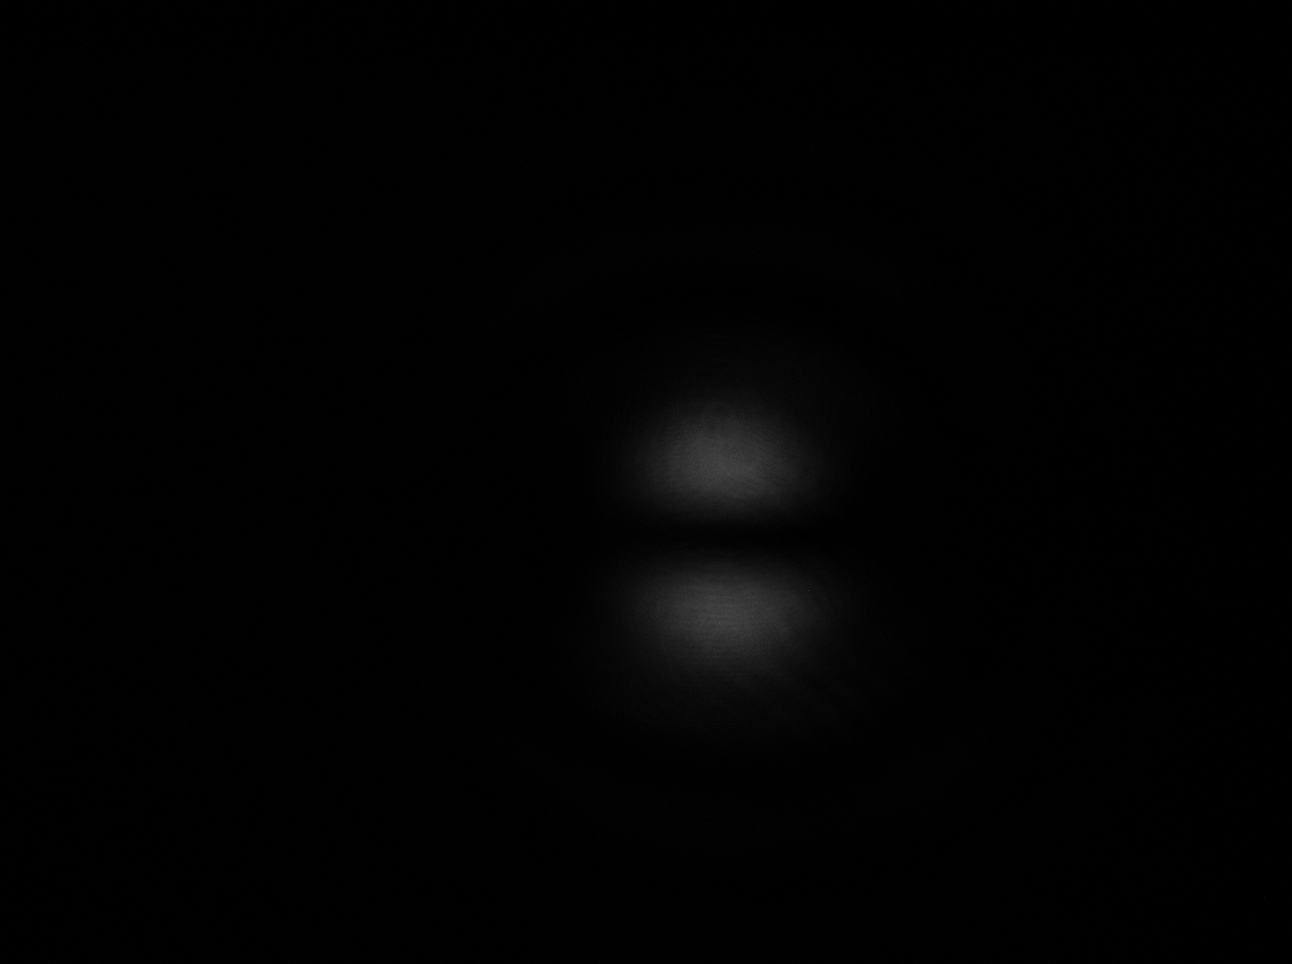
\includegraphics[width=0.9\textwidth]{./fig/1_1.png}
        \caption{检偏器$0^{\circ}$,径向偏振}
    \end{minipage}
    \begin{minipage}[b]{0.45\textwidth}
        \centering
        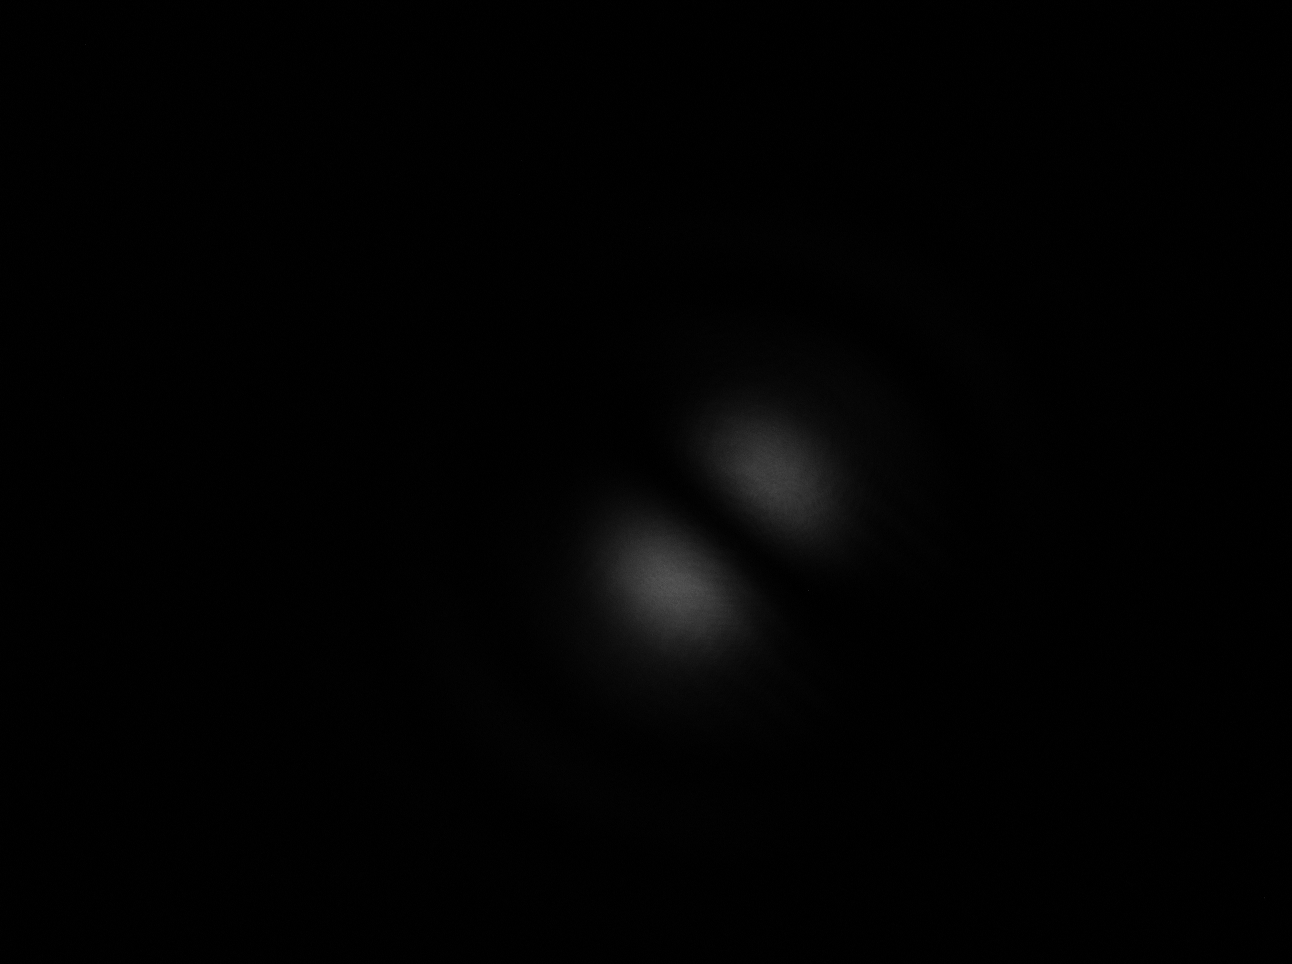
\includegraphics[width=0.9\textwidth]{./fig/1_4.png}
        \caption{检偏器$45^{\circ}$,径向偏振}
    \end{minipage}
\end{figure}

\begin{figure}[H]
    \centering
    \begin{minipage}[b]{0.45\textwidth}
        \centering
        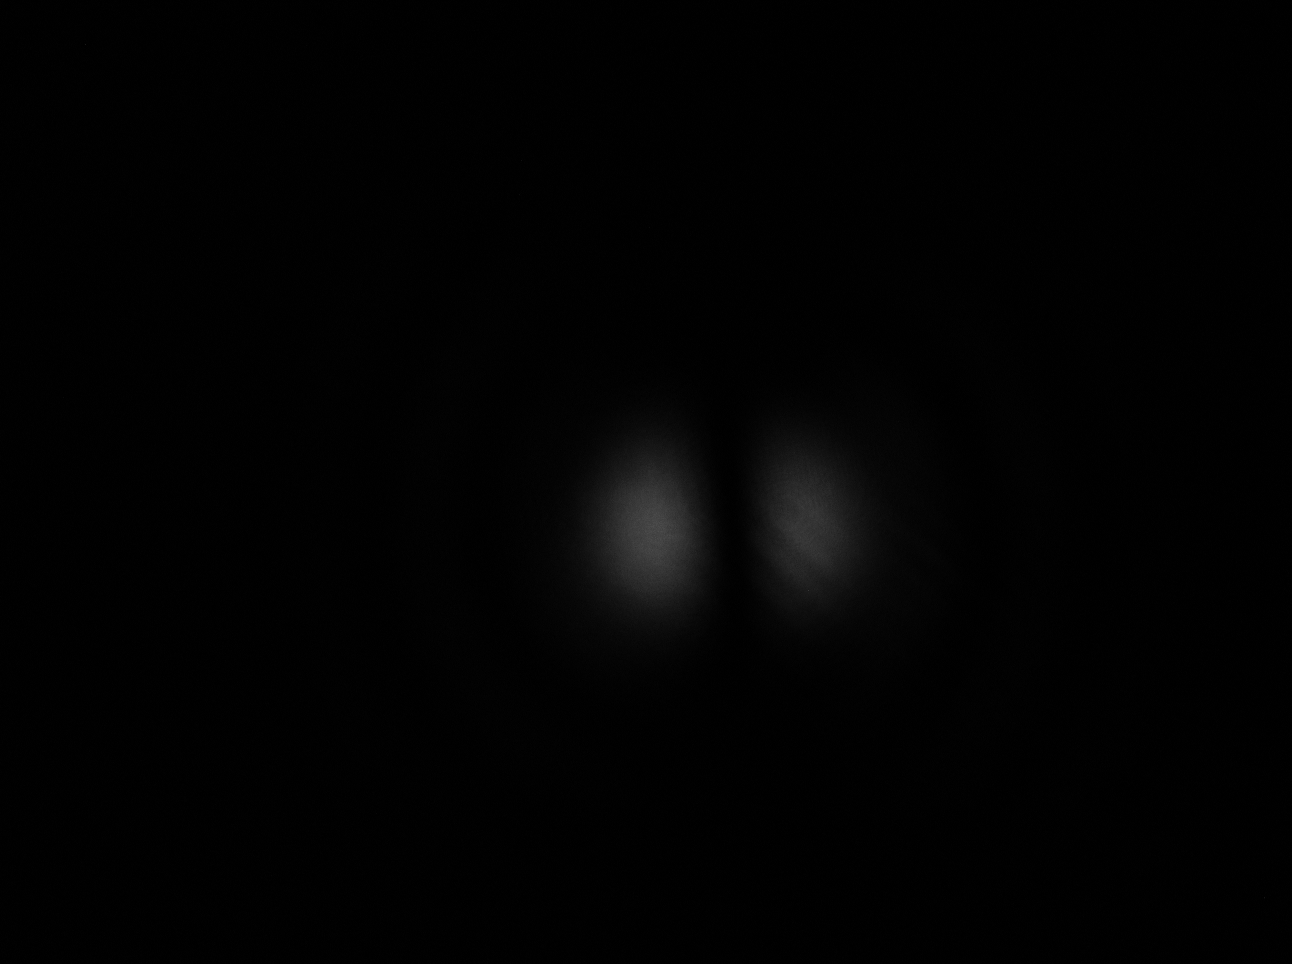
\includegraphics[width=0.9\textwidth]{./fig/1_3.png}
        \caption{检偏器$90^{\circ}$,径向偏振}
    \end{minipage}
    \begin{minipage}[b]{0.45\textwidth}
        \centering
        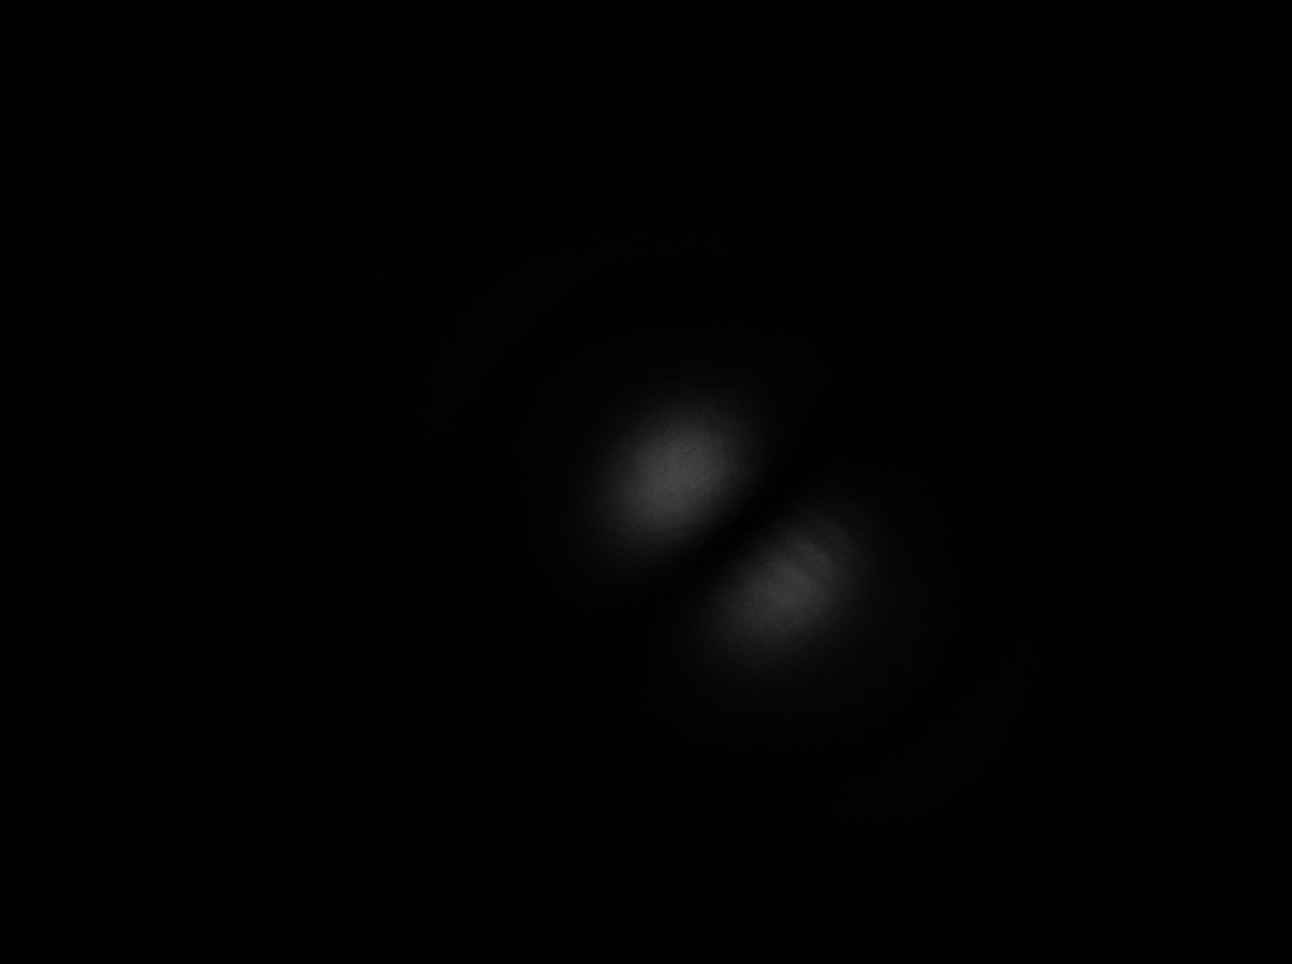
\includegraphics[width=0.9\textwidth]{./fig/1_2.png}
        \caption{检偏器$135^{\circ}$,径向偏振}
    \end{minipage}
\end{figure}

\subsection{角向偏振光检偏}

\begin{figure}[H]
    \centering
    \begin{minipage}[b]{0.45\textwidth}
        \centering
        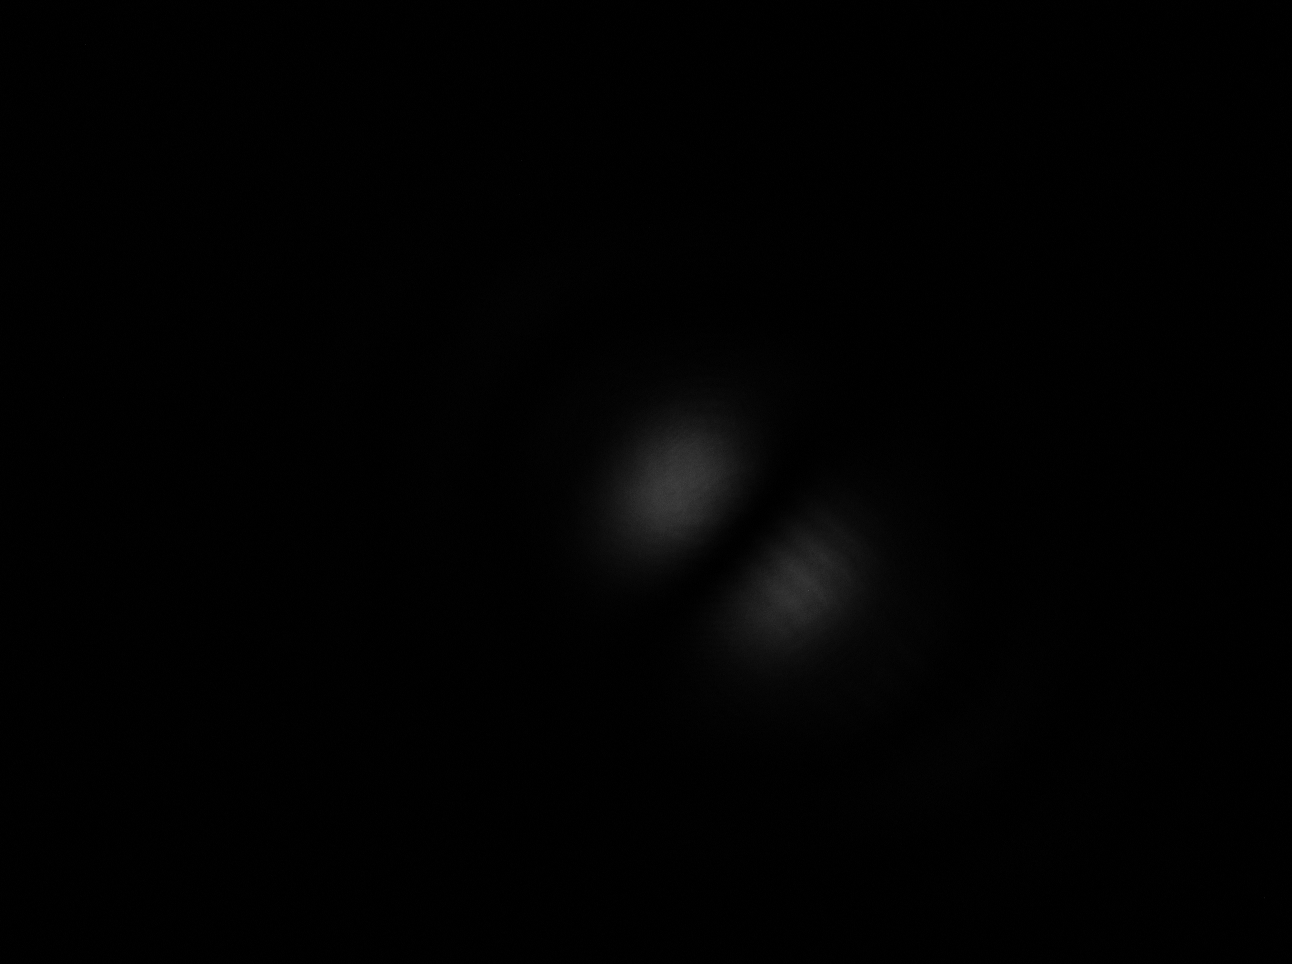
\includegraphics[width=0.9\textwidth]{./fig/1_5.png}
        \caption{检偏器$0^{\circ}$,角向偏振}
    \end{minipage}
    \begin{minipage}[b]{0.45\textwidth}
        \centering
        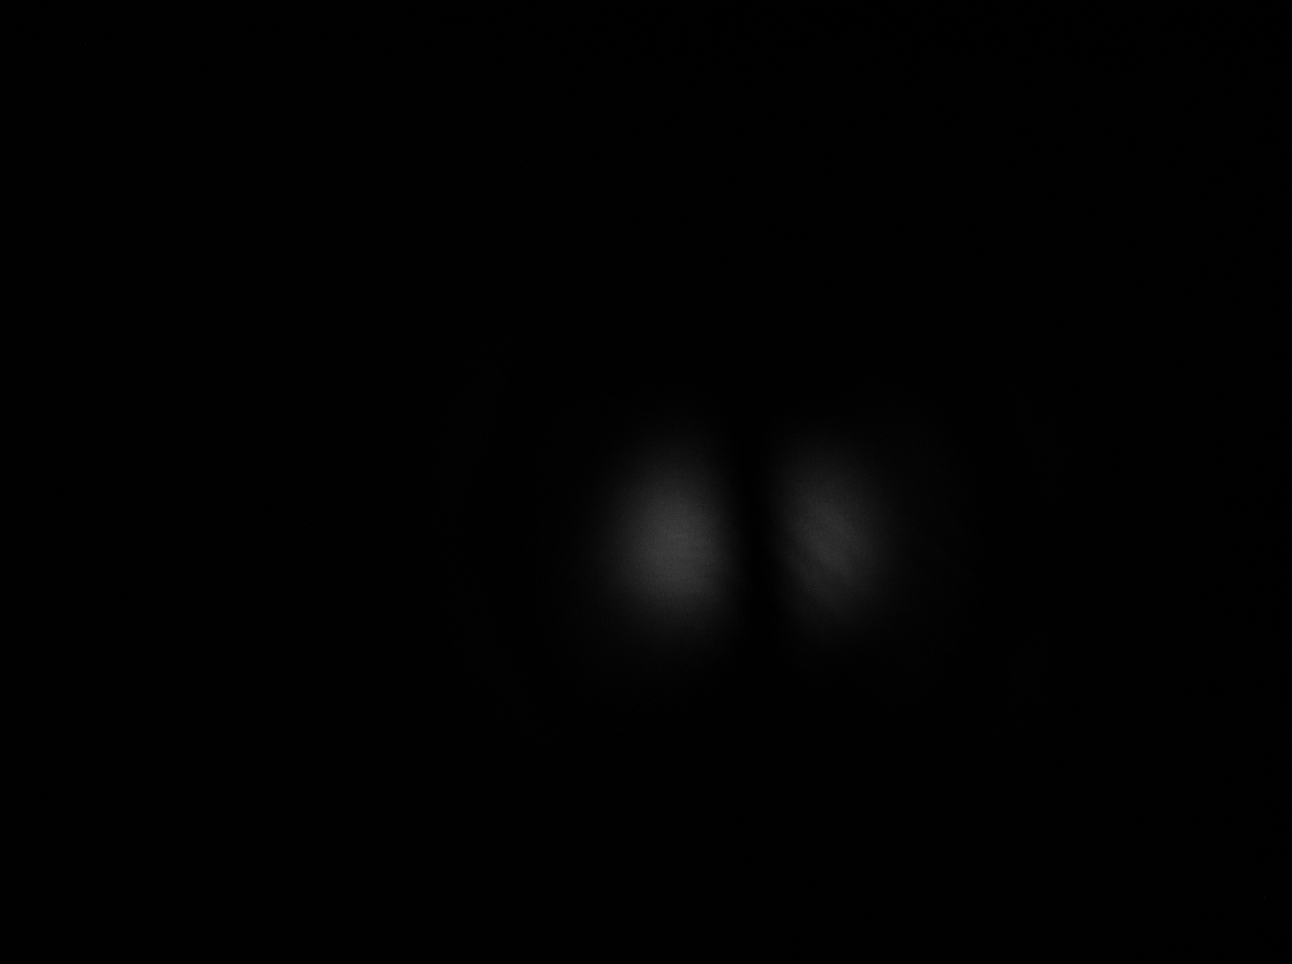
\includegraphics[width=0.9\textwidth]{./fig/1_8.png}
        \caption{检偏器$45^{\circ}$,角向偏振}
    \end{minipage}
\end{figure}

\begin{figure}[H]
    \centering
    \begin{minipage}[b]{0.45\textwidth}
        \centering
        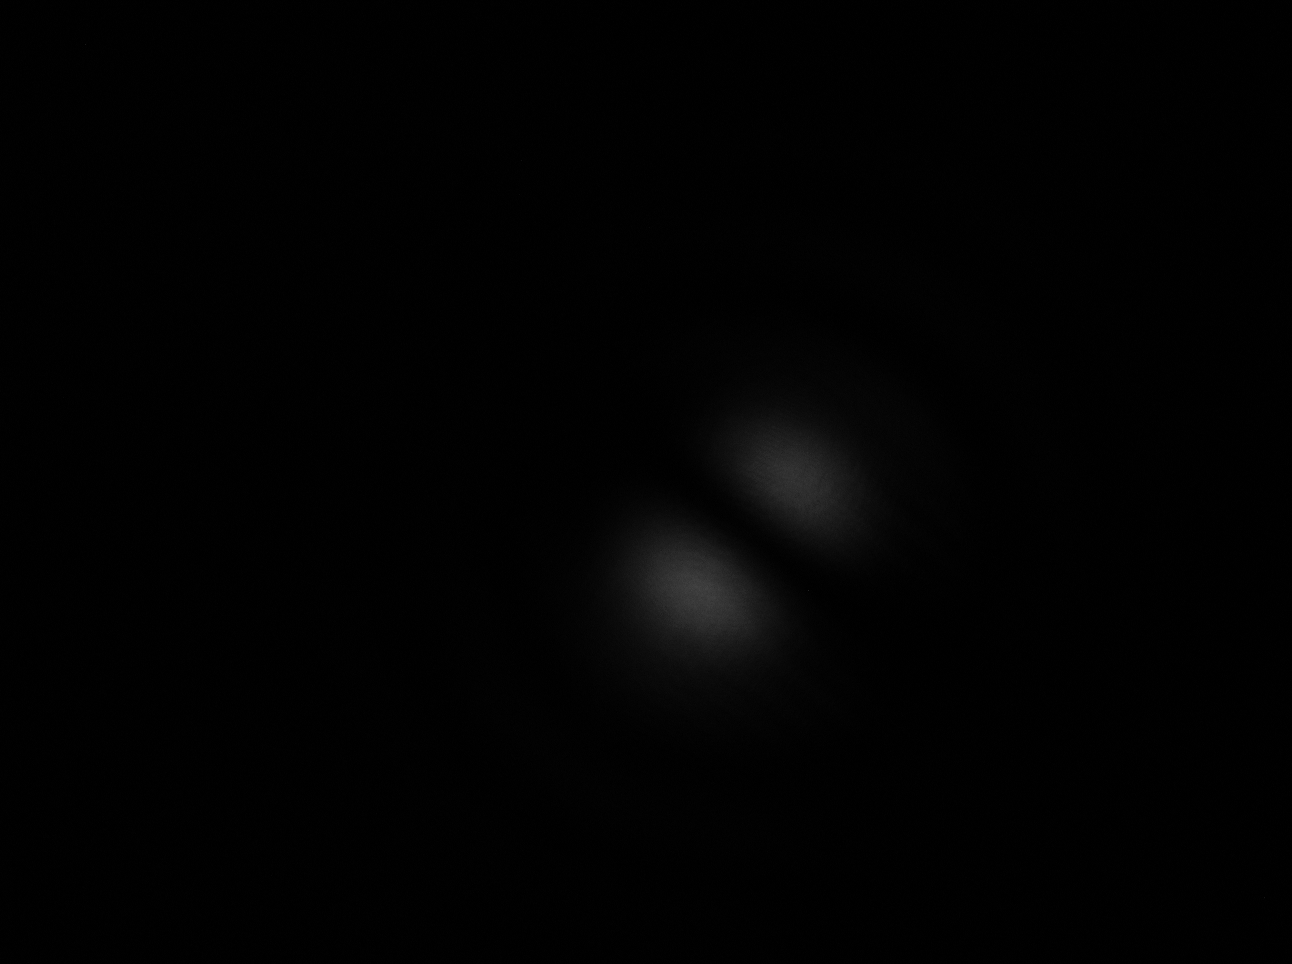
\includegraphics[width=0.9\textwidth]{./fig/1_7.png}
        \caption{检偏器$90^{\circ}$,角向偏振}
    \end{minipage}
    \begin{minipage}[b]{0.45\textwidth}
        \centering
        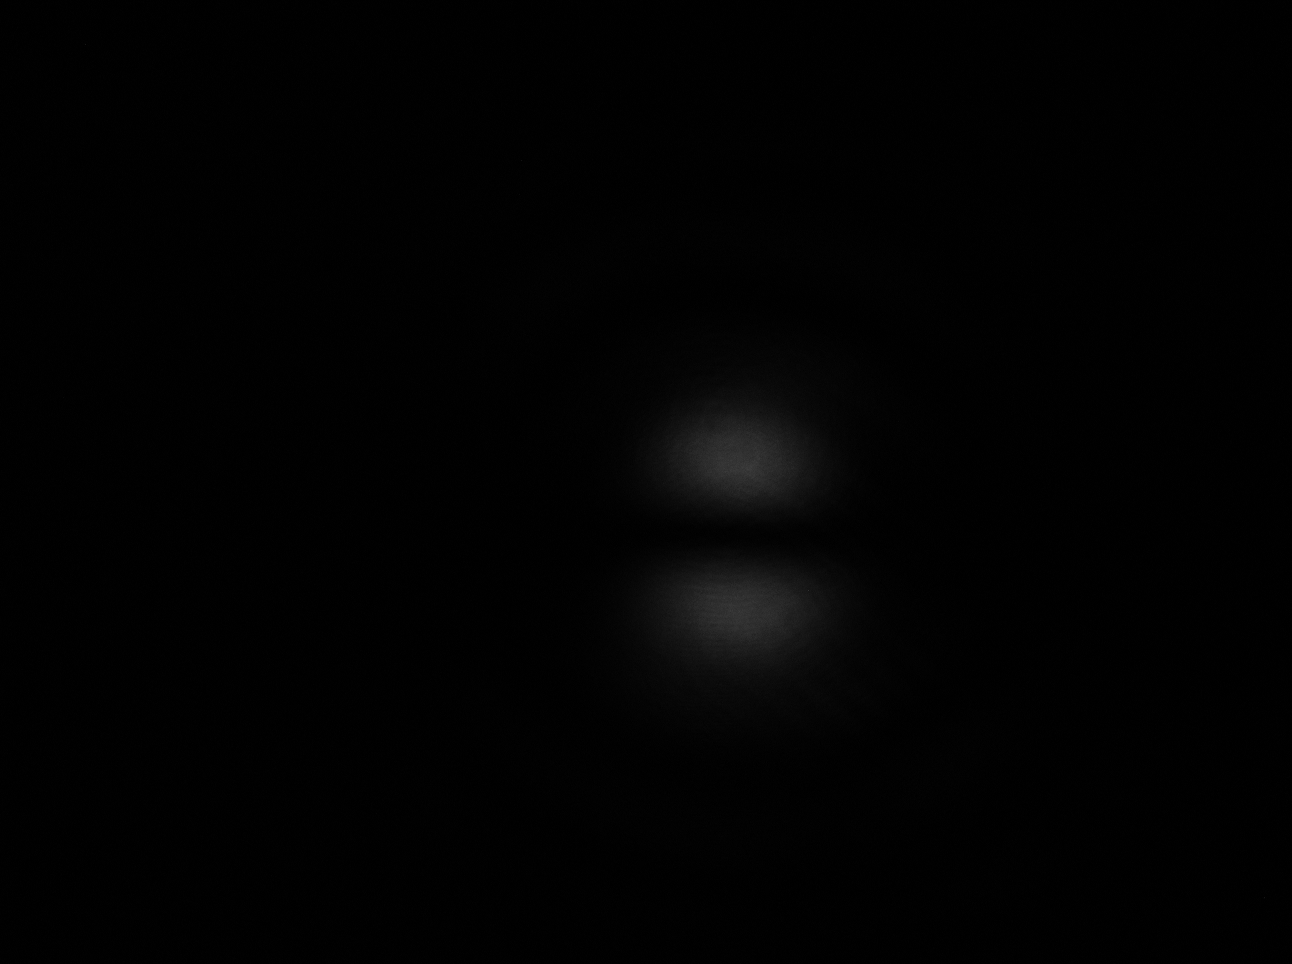
\includegraphics[width=0.9\textwidth]{./fig/1_6.png}
        \caption{检偏器$135^{\circ}$,角向偏振}
    \end{minipage}
\end{figure}

\section{二阶矢量光束光强分布}

\begin{figure}[H]
    \centering
    \begin{minipage}[b]{0.9\textwidth}
        \centering
        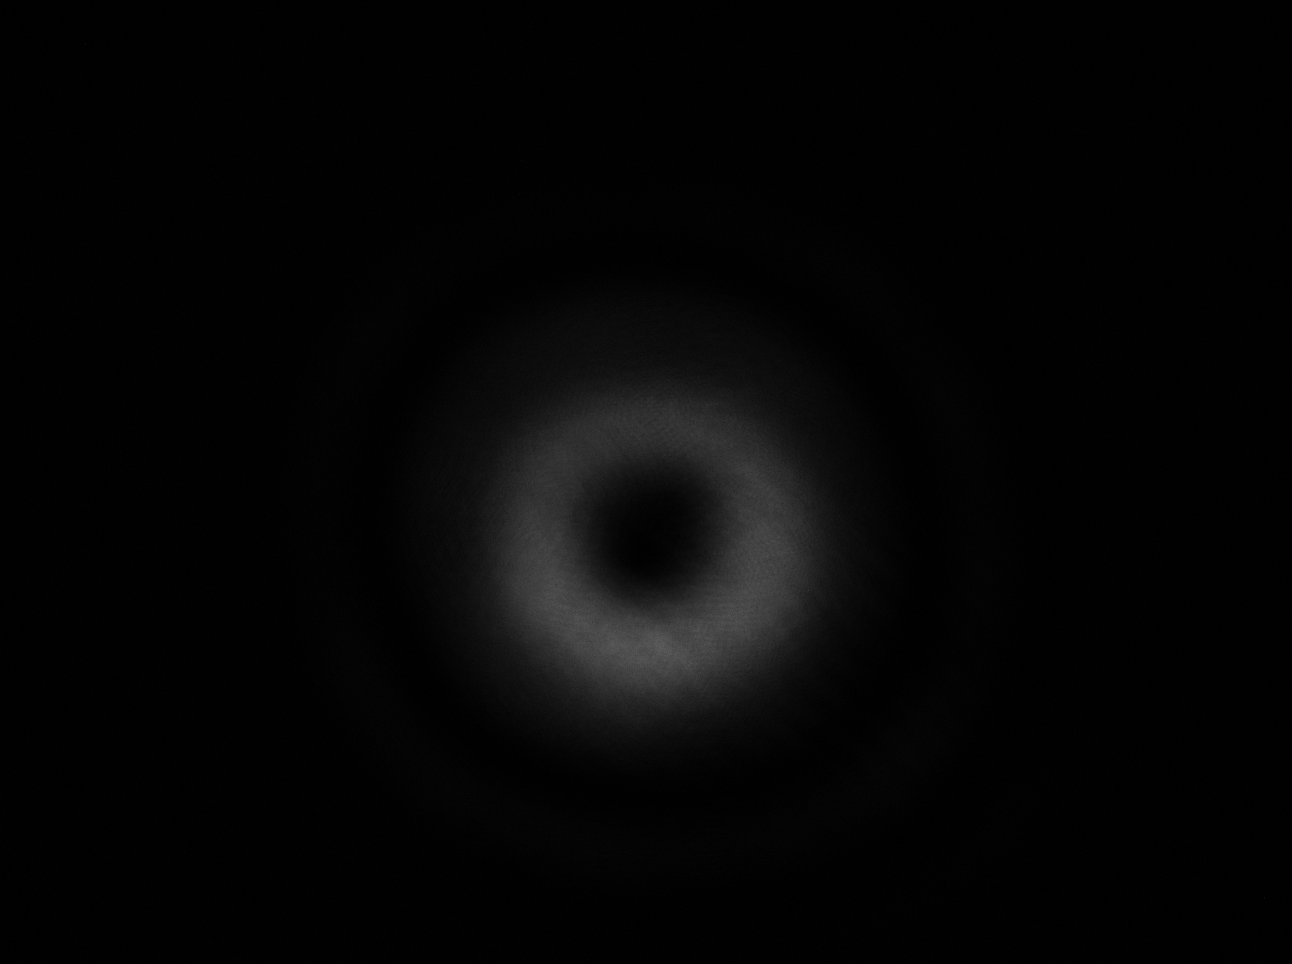
\includegraphics[width=0.7\textwidth]{./fig/2.png}
        \caption{二阶矢量光束光强分布}
    \end{minipage}
\end{figure}

\subsection{二阶矢量光束检偏}

\begin{figure}[H]
    \centering
    \begin{minipage}[b]{0.45\textwidth}
        \centering
        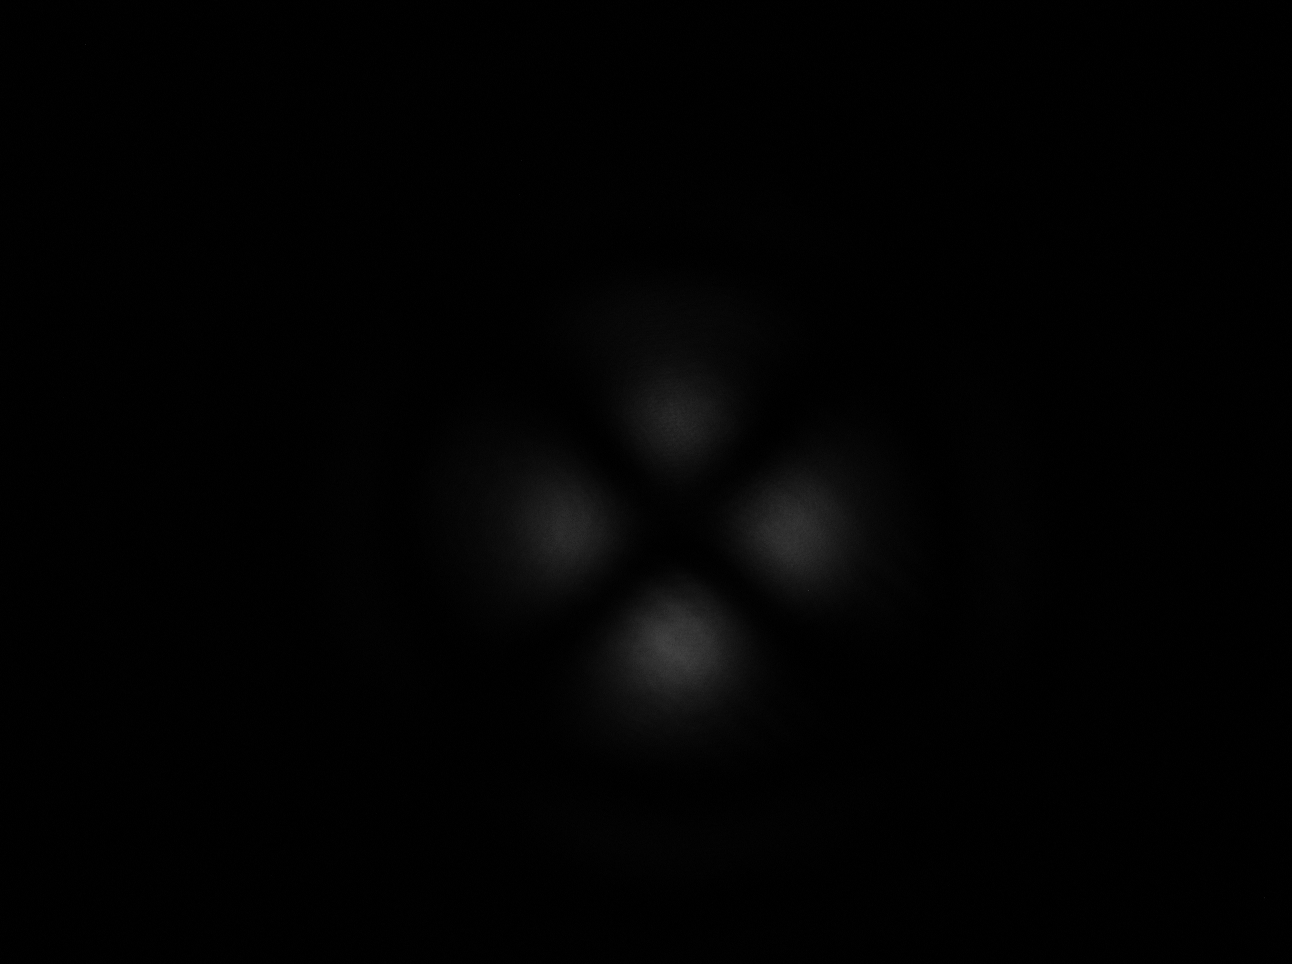
\includegraphics[width=0.9\textwidth]{./fig/2_1.png}
        \caption{检偏器$0^{\circ}$}
    \end{minipage}
    \begin{minipage}[b]{0.45\textwidth}
        \centering
        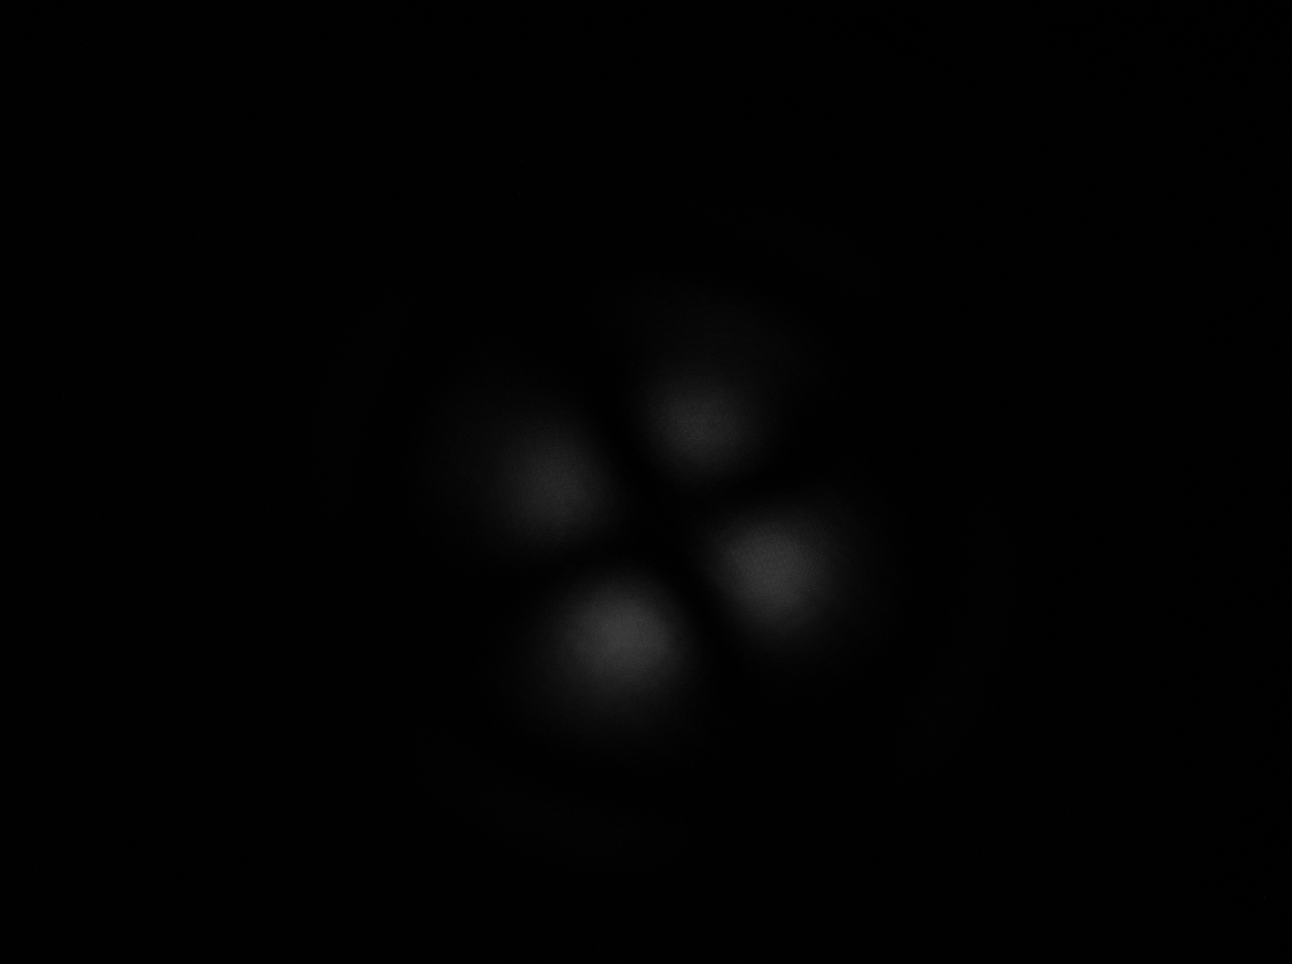
\includegraphics[width=0.9\textwidth]{./fig/2_4.png}
        \caption{检偏器$22.5^{\circ}$}
    \end{minipage}
\end{figure}

\begin{figure}[H]
    \centering
    \begin{minipage}[b]{0.45\textwidth}
        \centering
        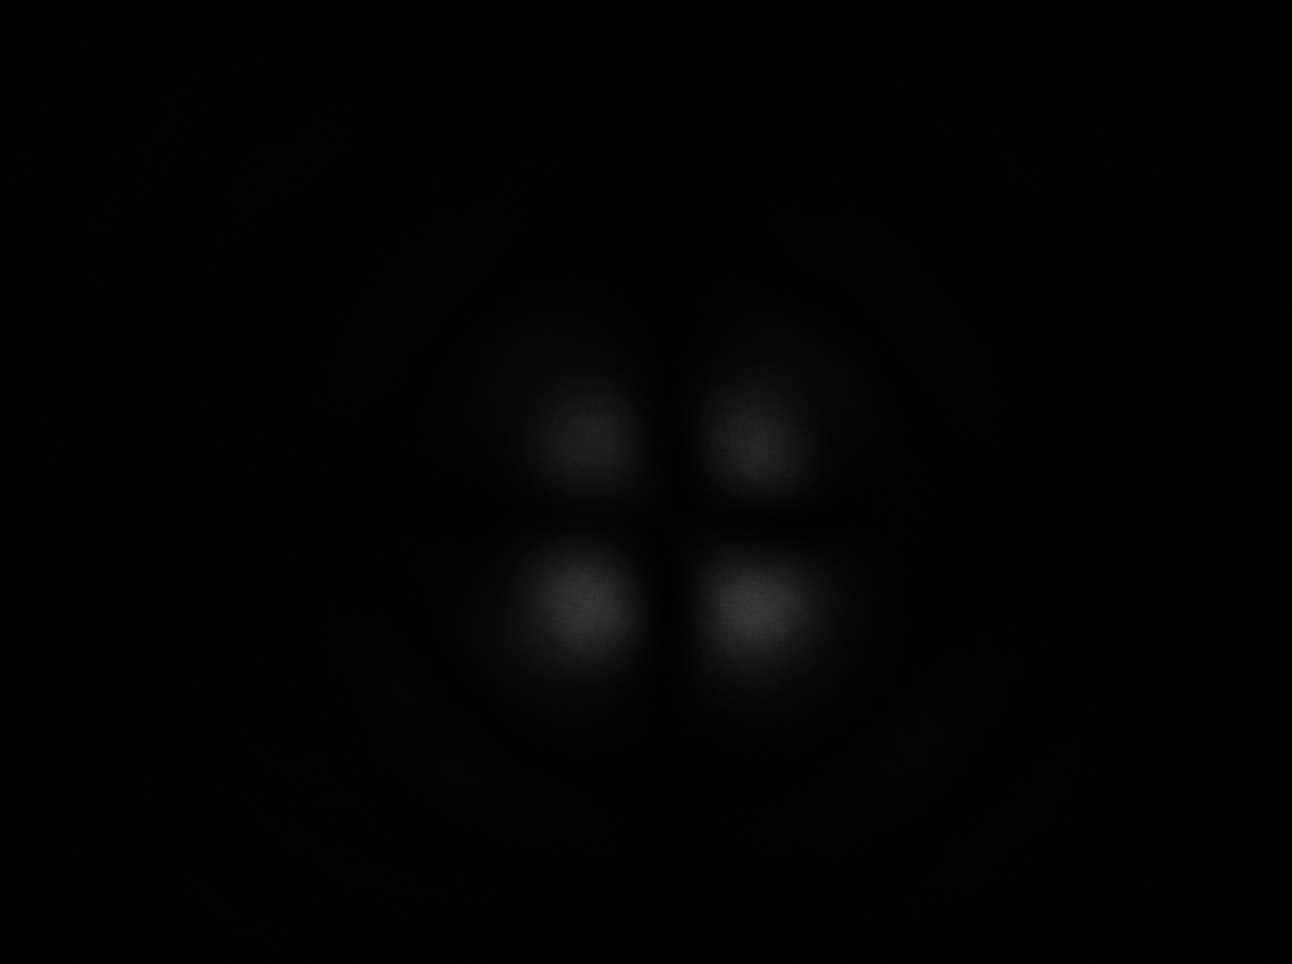
\includegraphics[width=0.9\textwidth]{./fig/2_3.png}
        \caption{检偏器$45^{\circ}$}
    \end{minipage}
    \begin{minipage}[b]{0.45\textwidth}
        \centering
        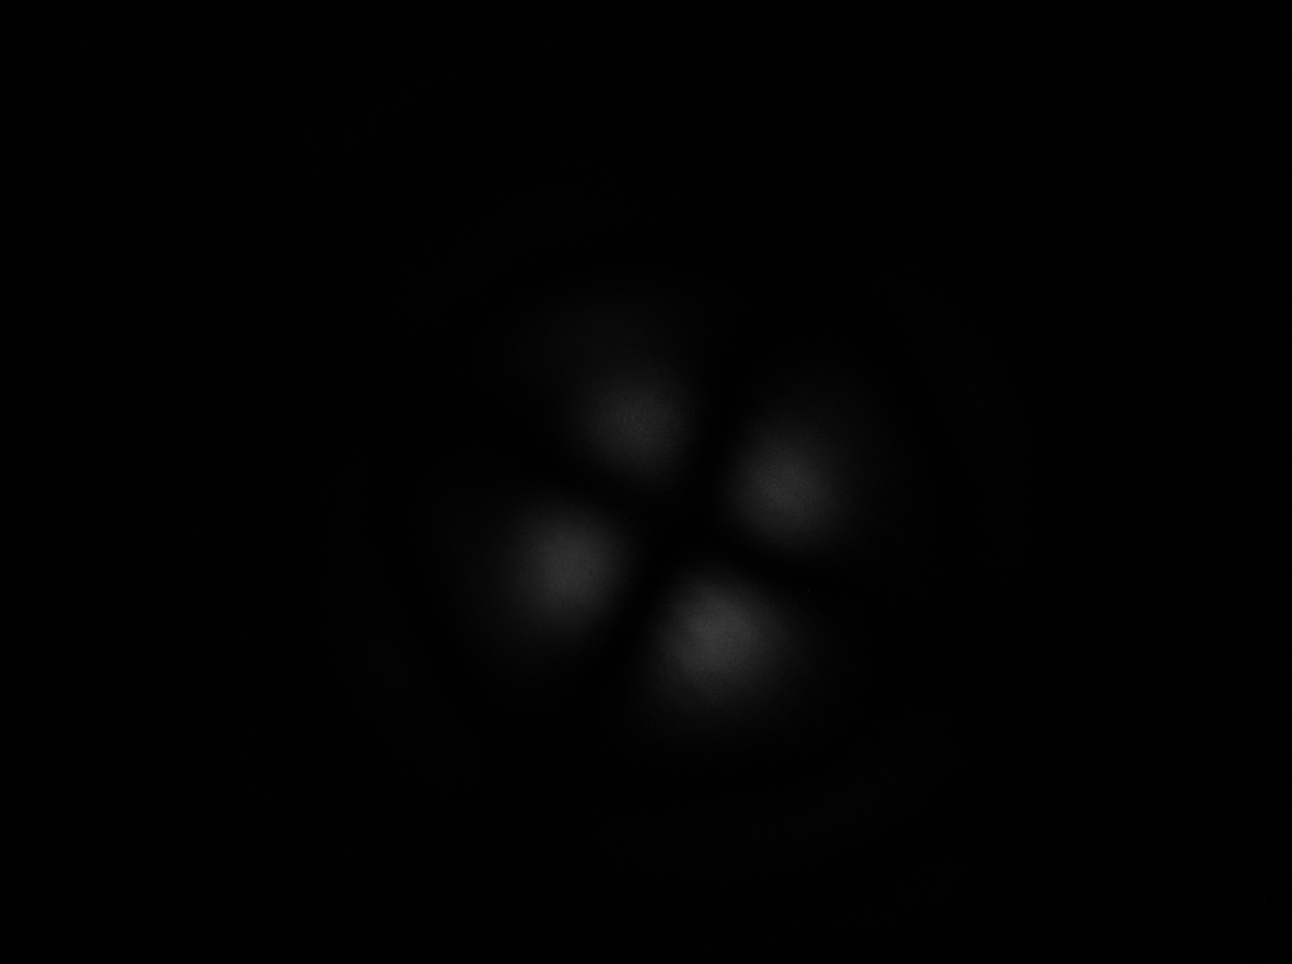
\includegraphics[width=0.9\textwidth]{./fig/2_2.png}
        \caption{检偏器$67.5^{\circ}$}
    \end{minipage}
\end{figure}

\section{一阶相位涡旋光束光强分布及相位检测}

\begin{figure}[H]
    \centering
    \begin{minipage}[b]{0.45\textwidth}
        \centering
        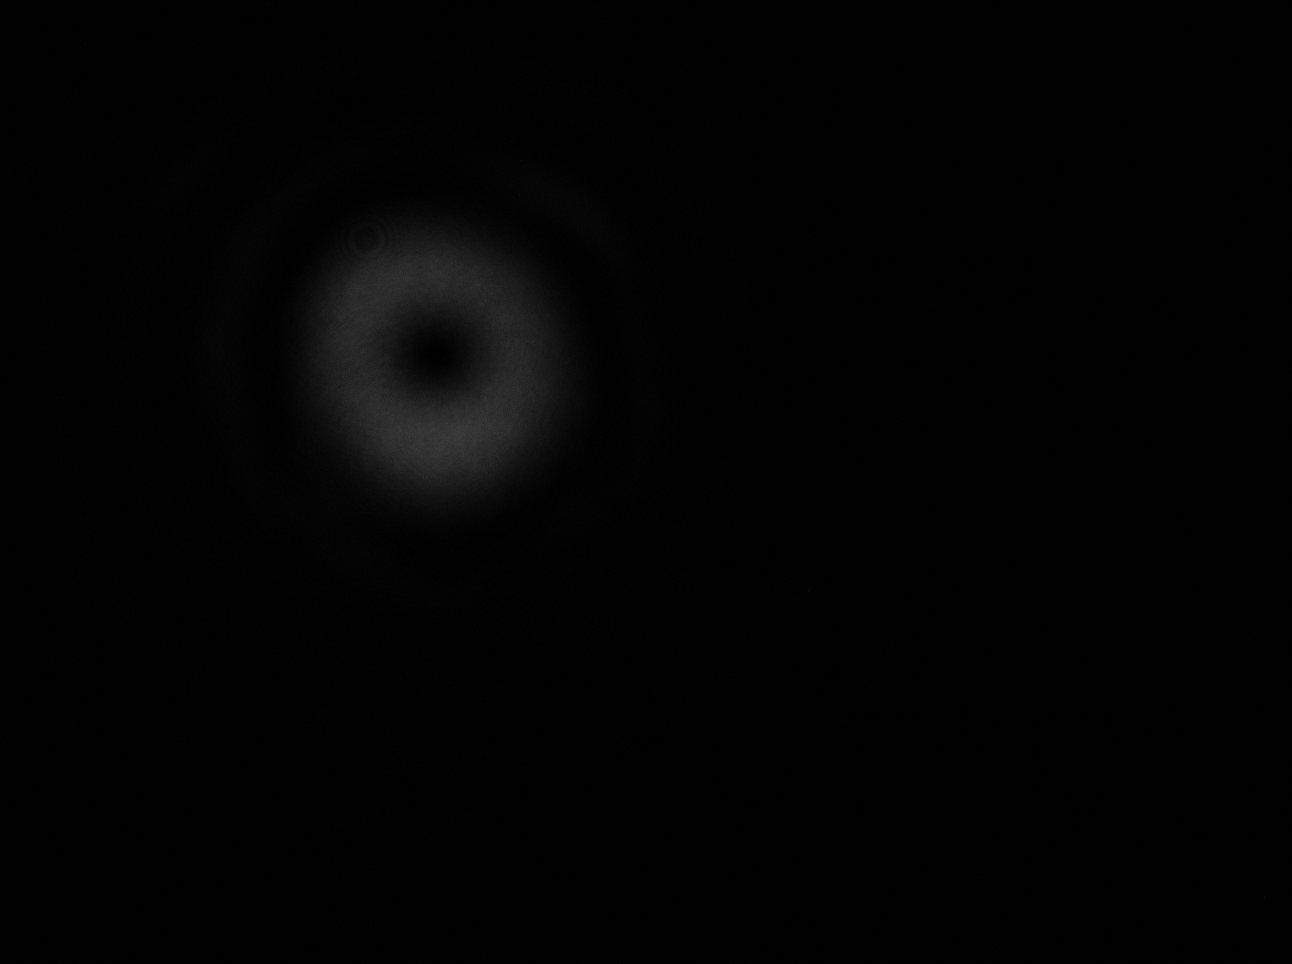
\includegraphics[width=0.9\textwidth]{./fig/3.png}
        \caption{一阶相位涡旋光束光强分布}
    \end{minipage}
    \begin{minipage}[b]{0.45\textwidth}
        \centering
        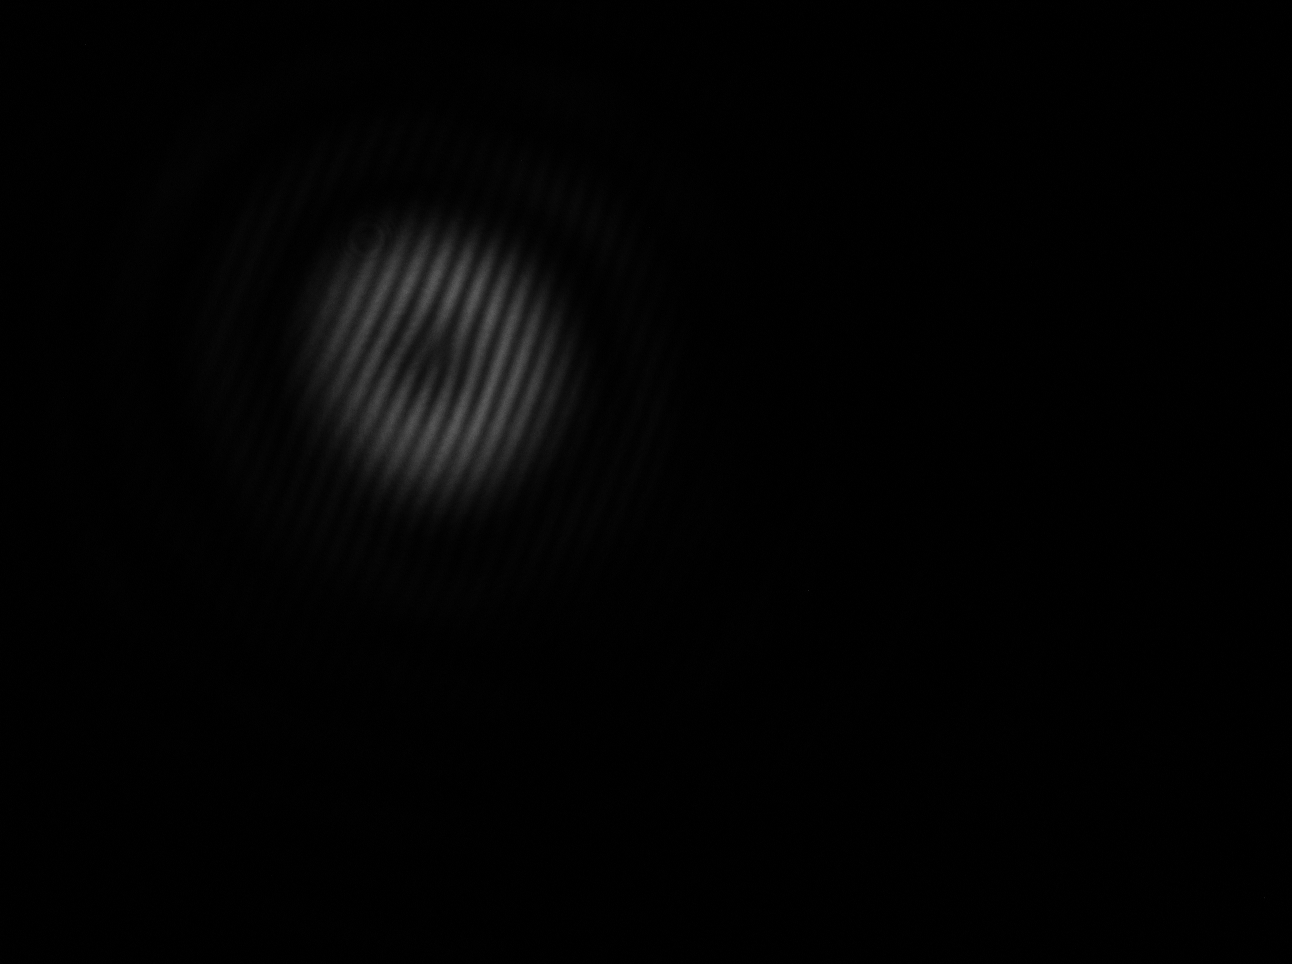
\includegraphics[width=0.9\textwidth]{./fig/3_1.png}
        \caption{一阶相位涡旋光束相位检测}
    \end{minipage}
\end{figure}


\section{二阶相位涡旋光束光强分布及相位检测}

\begin{figure}[H]
    \centering
    \begin{minipage}[b]{0.45\textwidth}
        \centering
        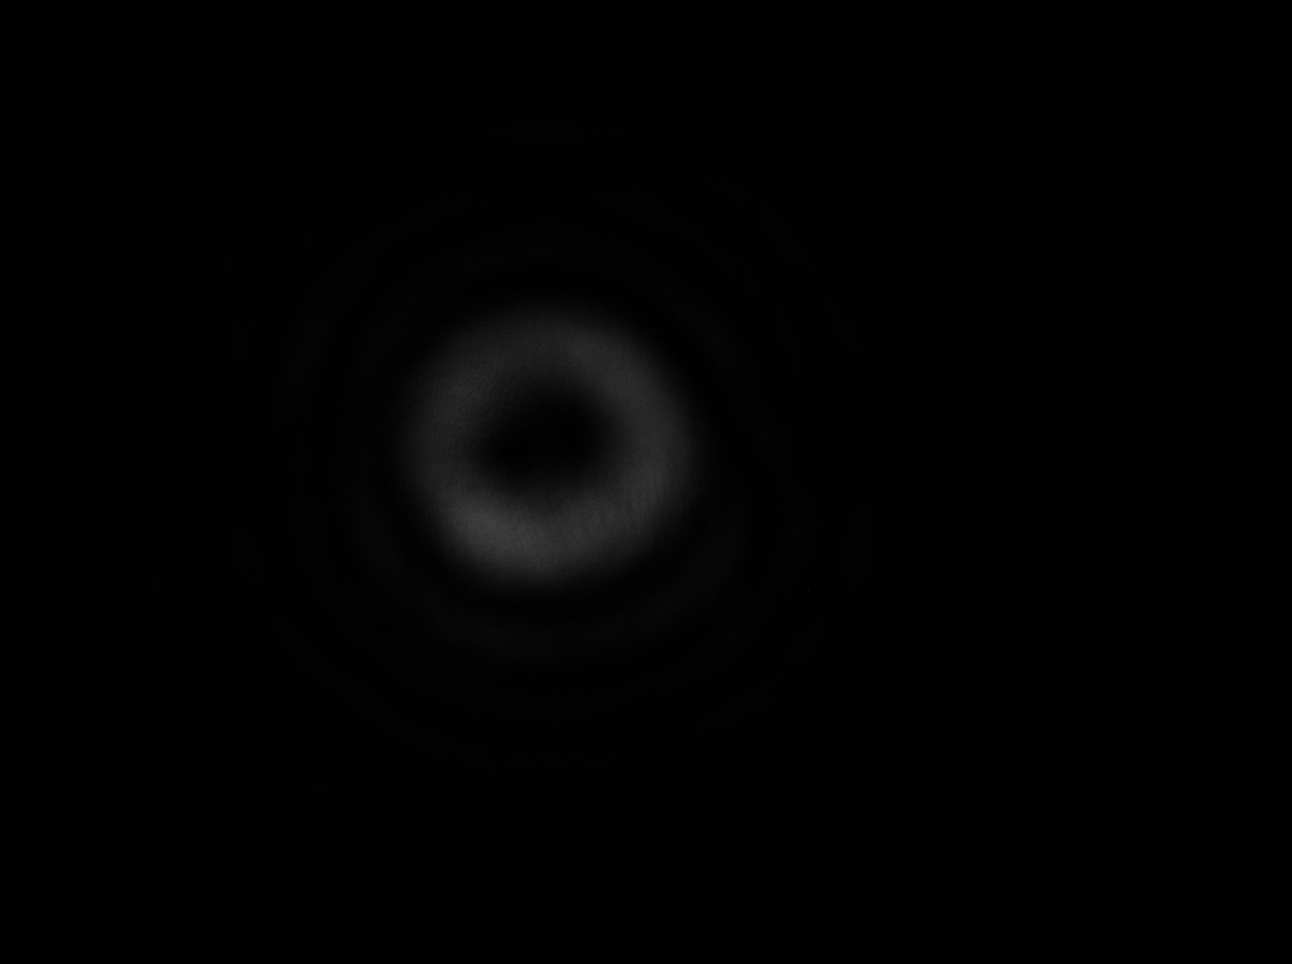
\includegraphics[width=0.9\textwidth]{./fig/4.png}
        \caption{二阶相位涡旋光束光强分布}
    \end{minipage}
    \begin{minipage}[b]{0.45\textwidth}
        \centering
        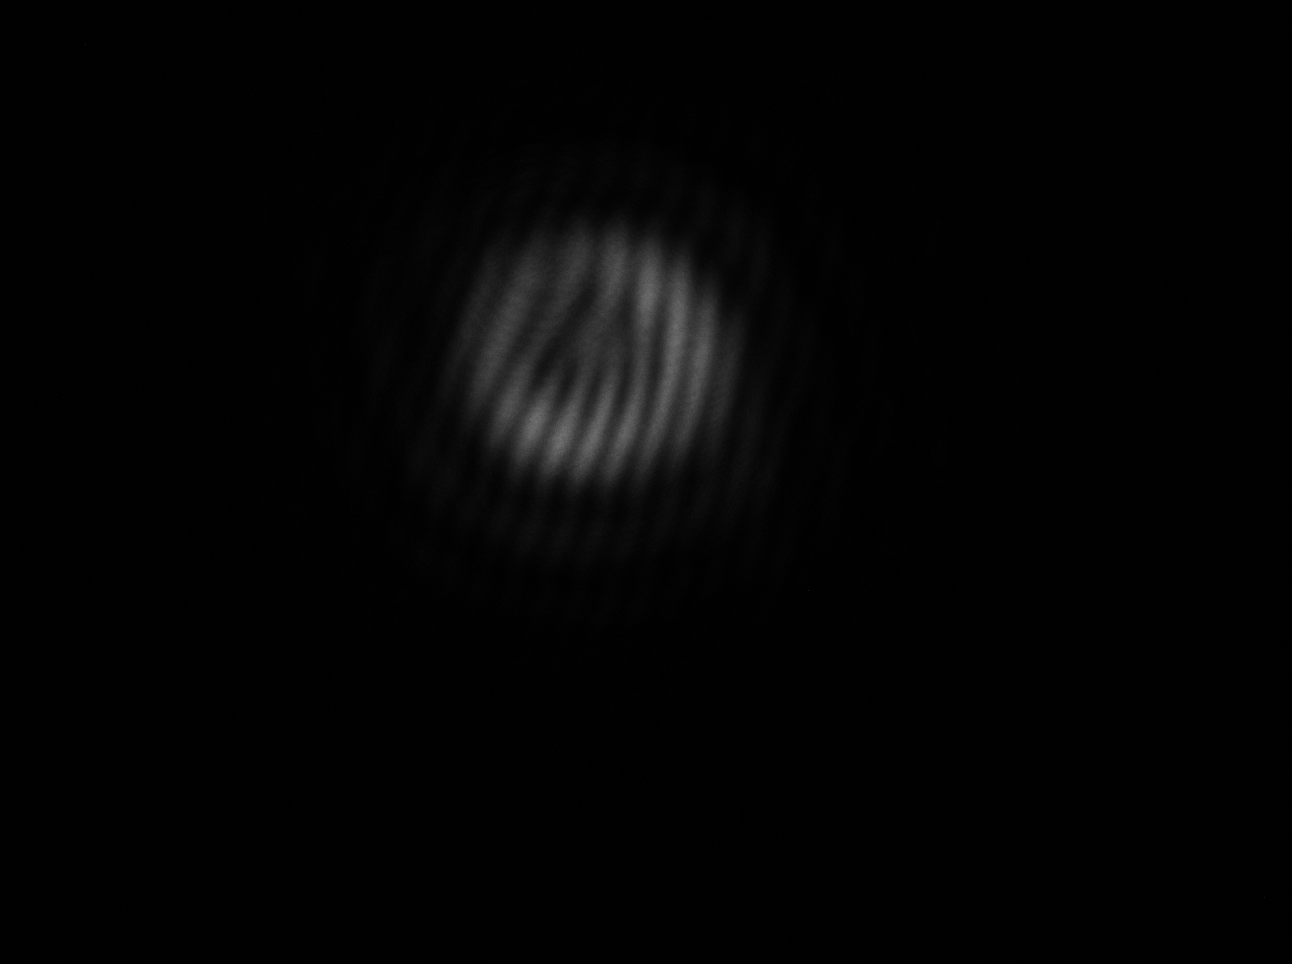
\includegraphics[width=0.9\textwidth]{./fig/4_1.png}
        \caption{二阶相位涡旋光束相位检测}
    \end{minipage}
\end{figure}

\end{document}